\documentclass{beamer}

%%%% Packages
\usepackage{amsmath, amsthm, amssymb}
\usepackage{array}              % for >{} in table column
                                % specification
\usepackage{algpseudocode}      % algorithmic environment

\usepackage[english]{babel}
\usepackage{color}              % for color definition
\usepackage{xcolor}
\usepackage{graphicx}           % for including images
\usepackage{multirow}           % for multirow
\usepackage{tabularx}           % for centering in table
\usepackage{relsize}
% TIKZ setup for drawing graphs
\usepackage{tikz}
\usetikzlibrary{arrows}
\usetikzlibrary{positioning}
% \pgfkeysalso doesn't change the path
\tikzset{onslide/.code args={<#1>#2}{ \only<#1>{\pgfkeysalso{#2}} }}
% \pgfkeysalso doesn't change the path
\tikzset{temporal/.code args={<#1>#2#3#4}{
    \temporal<#1>{\pgfkeysalso{#2}}{\pgfkeysalso{#3}}{\pgfkeysalso{#4}}
}}
\tikzset{fontscale/.style = {font=\relsize{#1}}
    }
\tikzstyle{highlight}=[red,ultra thick]

%%%% Macros and Definitions
\definecolor{firebrick4}{RGB}{139,026,026}
\definecolor{gray57}{RGB}{145,145,145}
\definecolor{gray71}{RGB}{181,181,181}
\definecolor{gray84}{RGB}{212,212,212}
\definecolor{lightcyan4}{RGB}{122,139,139}
\definecolor{dodgerblue4}{RGB}{16,78,139}
\definecolor{dodgerblue3}{RGB}{24,116,205}

\setcounter{tocdepth}{1}

\newlength{\picwidth}
\setlength{\picwidth}{2.5cm}
\newlength{\picheight}
\setlength{\picheight}{2cm}

\newlength{\firstcolumnwidth}
\setlength{\firstcolumnwidth}{0.25\textwidth}
\newlength{\mycolumnwidth}
\setlength{\mycolumnwidth}{0.13\textwidth}

%%%% Presentation Setup
\mode<presentation>
{
  \usetheme{Ilmenau}
  \usecolortheme{beaver}
  \usefonttheme[onlylarge]{structuresmallcapsserif}
}
\setbeamercolor{title}{fg=dodgerblue4}
\setbeamercolor{frametitle}{fg=dodgerblue4}
\setbeamercolor*{palette secondary}{fg=dodgerblue4,bg=gray84}
\setbeamercolor*{palette tertiary}{fg=white,bg=dodgerblue4}
\setbeamercolor*{item}{fg=dodgerblue4}
\setbeamercolor{alerted text}{fg=red}

\setbeamerfont{author}{size=\scriptsize}
\setbeamerfont{institute}{size=\scriptsize}
\setbeamerfont{date}{size=\tiny}
\setbeamerfont{normal text}{size=\scriptsize}

\beamertemplatenavigationsymbolsempty

%%%% Title
\title[]{Markov Logic Network}
\author[Sidorenko]{Wladimir Sidorenko\\ \texttt{uladzimir.sidarenka{@}uni-potsdam.de}}
\institute{University of Potsdam}
\date{\today}

\pgfdeclareimage[interpolate=true,height=2.5cm]{logo}{img/uni_potsdam_logo.png}
\titlegraphic{\pgfuseimage{logo}}

%%%% Document
\begin{document}
%%%%%%%%%%%%%%%%%%%%%%%%%%%%%%%%%%%%%%%%%%%%%%%%%%%%%%%%%%%%%%%%%%
%%% Title Page
\begin{frame}{}
  \titlepage
\end{frame}

%%%%%%%%%%%%%%%%%%%%%%%%%%%%%%%%%%%%%%%%%%%%%%%%%%%%%%%%%%%%%%%%%%
%%% Task Definition and Experiment Setup
\section{Introduction}
\subsection{First-order Logic}
\begin{frame}{\insertsubsection}
  \begin{definition}
    First-order logic (FOL) is a symbolized reasoning system
    consisting of sentences, or formulae, in which each formula
    defines some properties or relations of a particular object in the
    given domain.
  \end{definition}
  A formula in FOL can be composed of the following elements:
  \begin{itemize}
    \item \textbf{constants} which represent objects in the domain of
      interest, e.g. \texttt{Anna}, \texttt{Bob};
    \item \textbf{variables} which are symbols that range over the
      objects in the domain, e.g. \texttt{x}, \texttt{y};
    \item \textbf{function symbols} which represent mappings from
      tuples of objects to objects, e.g. \texttt{ParentsOf(Anna)};
    \item \textbf{predicate symbols} which represent relations among
      objects in the domain, e.g. \texttt{Brother(Bob, Anna)}.
  \end{itemize}
\end{frame}

\begin{frame}{\insertsubsection}
A \textbf{term} in FOL is any expression representing an object in the
domain. It can be a constant, a variable, or a function applied to a
tuple of terms.  A \textbf{ground term} is a term containing no
variables, e.g. \texttt{Anna} or \texttt{SiblingsOf(Anna)}.\vspace{0.5cm}

A predicate symbol applied to a tuple of terms is called an
\textbf{atomic formula} or \textbf{atom}.  Correspondingly, an atomic
formula all of whose arguments are ground terms is called a
\textbf{ground atom}, e.g. \texttt{IsSchoolgirl(Anna)}.\vspace{0.5cm}

A \textbf{possible world} is a conjunction of all formulae specified
in the knowledge base for the domain in which every ground atom is
assigned a truth value.
\end{frame}

\begin{frame}[fragile]{First-order Logic}
An important property of possible worlds is the ability to infer the
\textbf{satisfiability} of new formulae which are not in the knowledge
base given that the knowledge base world is satisfiable.\vspace{0.5cm}

If a satisfiable knowledge base $KB$ exists and it does not contain a
formula $F$, we can infer that $F$ is true if the conjunction $KB \cup
\neg F$ is not satisfiable.
\end{frame}

\begin{frame}{\insertsubsection}
Drawbacks of FOL:
\begin{itemize}
  \item The satisfiability problem is a well-known NP-complete problem
    and therefore intractable to solve even for moderately big
    knowledge bases.  And if we cannot prove that a $KB$ is
    satisfiable, we cannot do the inference;
    \visible<3->{\textbf{Approximate.}}

  \item Formulae in FOL are hard constraints, a world which violates
    at least one formula is not allowed to exist.  The real world is,
    however, less categorical; \visible<3->{\textbf{Add probabilities to formulae.}}
\end{itemize}
\visible<2->{How can these drawbacks be solved?}
\end{frame}

\subsection{Markov Network}
\begin{frame}{\insertsubsection}
  \begin{definition}
    \textbf{Markov network} (or Markov Random Field) is an undirected
    probabilistic graphical model whose nodes represent random
    variables and edges between nodes represent relations between
    those variables.
  \end{definition}
  \begin{example}
    \begin{center}
      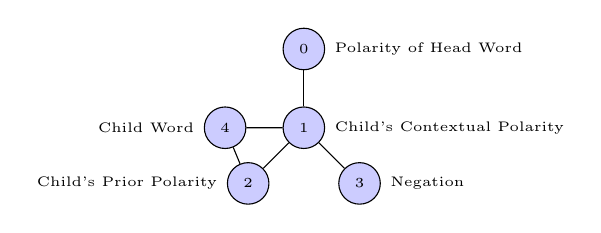
\begin{tikzpicture}
        [auto=left,scale=0.6,
          every node/.style={circle,draw,fill=blue!20,minimum size=15pt},
          every label/.style={shape=rectangle,draw=none,fill=none}]
        \node[align=center,label={0:\tiny Polarity of Head Word}] (n0) {\tiny 0};
        \node (n1) [below of=n0,label={0:\tiny Child's Contextual Polarity}] {\tiny 1};
        \node (n2) [below left of=n1,label={180:\tiny Child's Prior Polarity}] {\tiny 2};
        \node (n3) [below right of=n1,label={0:\tiny Negation}] {\tiny 3};
        \node (n4) [left of=n1,label={180:\tiny Child Word}] {\tiny 4};
        \foreach \from/\to in {n0/n1,n1/n2,n1/n3,n4/n2,n4/n1}
        \draw (\from) -- (\to);
      \end{tikzpicture}
    \end{center}
  \end{example}
\end{frame}

\begin{frame}{Markov Properties}
  \scriptsize All variables (nodes) of an MRF should satisfy the following
  three properties:
  \begin{itemize}
    \item<2-> \textbf{Pairwise Markov property} - any two non-adjacent
      variables are conditionally independent given all other
      variables;
    \item<3-> \textbf{Local Markov property} - a variable is conditionally
      independent of all other variables given its neighbors;
    \item<4-> \textbf{Global Markov property} - Any two subsets of
      variables are conditionally independent given a separating
      subset.
  \end{itemize}
  \begin{example}<1->
    \begin{center}
      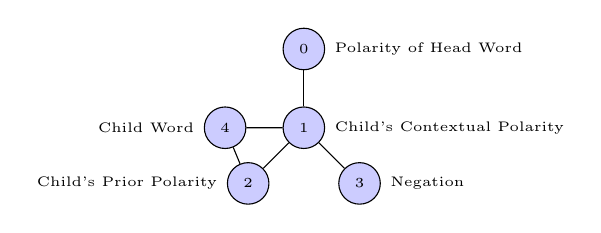
\begin{tikzpicture}
        [auto=left,scale=0.6,
          every node/.style={circle,draw,fill=blue!20,minimum size=15pt},
          every label/.style={shape=rectangle,draw=none,fill=none}]
        \node[align=center,onslide={<2-4>{red}},label={0:\tiny Polarity of Head Word}] (n0) {\tiny 0};
        \node (n1) [below of=n0,onslide={<2-4>{blue}},label={0:\tiny Child's Contextual Polarity}] {\tiny 1};
        \node (n2) [below left of=n1,onslide={<2-4>{red}},label={180:\tiny Child's Prior Polarity}] {\tiny 2};
        \node (n3) [below right of=n1,onslide={<2>{blue}},onslide={<3,4>{red}},label={0:\tiny Negation}] {\tiny 3};
        \node (n4) [left of=n1,onslide={<2,3>{blue}},onslide={<4>{red}},label={180:\tiny Child Word}] {\tiny 4};
        \foreach \from/\to in {n0/n1,n1/n2,n1/n3,n4/n2,n4/n1}
        \draw (\from) -- (\to);
      \end{tikzpicture}
    \end{center}
  \end{example}
  \pause
\end{frame}

\begin{frame}{Joint Probability Distribution}
  The joint probability distribution (JPD) over a set of variables $X$
  is defined by a Markov Network model as:
  \begin{equation}
    P(X=x) = \frac{1}{Z}\prod_k\phi_k(x_{\{k\}})
  \end{equation}
  where

  $x$ - is a particular value assignment to the variables in $X$

  $Z$ - is the normalizing \textit{partition function} which is set to
  $Z_{x \in X}\prod_k\phi_k(x_{\{k\}})$

  $\phi_k$ - is a potential (non-negative real-valued) function of the
  state of $k$-th clique

  $x_k$ - is the state of $k$-th clique
\end{frame}

\begin{frame}{Joint Probability Distribution}
  Another way to define a JPD is as \textit{log-linear model}:
  \begin{equation}
    P(X=x) = \frac{1}{Z}\exp\Big(\sum_j(w_jf_j(x)\Big)
  \end{equation}
  where

  $f_j(x) \in {0, 1}$ - is a binary feature for each possible state $x_{k}$ of
  each clique

  $w_j$ - is the weight associated with the $j$-th state of
  corresponding clique and is usually set to $log\phi_k(x_k)$
\end{frame}

\section{Markov Logic Network}
\subsection{Definition}
\begin{frame}[fragile]{\insertsubsection}
  \begin{definition}
    A Markov logic network (MLN) $L$ is a set of pairs ($F_i$, $w_i$),
    where $F_i$ is a formula in first-order logic and $w_i$ is a real
    number.  Together with a finite set of constants $C = \{c_1, c_2,
    ..., c_{|C|}\}$, it defines a Markov network $M_{L,C}$ as follows:
      \begin{enumerate}
      \item $M_{L,C}$ contains one binary node for each possible
        grounding of each atom appearing in L.  The value of the node
        is 1 if the ground atom is true, and 0 otherwise.

      \item $M_{L,C}$ contains one feature for each possible grounding
        of each formula $F_i$ in $L$.  The value of this feature is 1
        if the ground formula is true, and 0 otherwise.  The weight of
        the feature is the $w_i$ associated with $F_i$ in
        L.\cite{Domingos-06}
      \end{enumerate}
  \end{definition}
\end{frame}

\subsection{Learning}
\begin{frame}{\insertsubsection}
\end{frame}

\subsection{Inference}
\begin{frame}{\insertsubsection}
\end{frame}


\section{Examples}
\subsection{Alchemy}
\begin{frame}{\insertsubsection}
Open-source software package available at\\
{\small\url{http://alchemy-2.googlecode.com/files/alchemy-2.tar.gz}}\vspace{0.5cm}

Key components:
\begin{itemize}
  \item learnwts
  \item infer
  \item learnstruct
\end{itemize}
\end{frame}

\subsection{Binomial Distribution}
\begin{frame}{\insertsubsection}
MLN:\\
\texttt{\small
  flip = \{1, ..., 20\}\\
  Heads(flip)\\
  0.5 Heads(f)
}\\
\vspace{0.5cm}
DB:\\
\texttt{EMPTY}\\
\vspace{0.5cm}
Inference:\\
\texttt{
  \small
  infer -i binomial.mln -r binomial.result  -e empty.db -q Heads}
\end{frame}

\subsection{Multinomial Distribution}
\begin{frame}{\insertsubsection}
MLN:\\
\texttt{\small
  throw = \{1, ..., 20\}\\
  face  = \{1, ..., 6\}\\
  Outcome(throw, face!)\\
  Outcome(t, +f)}\\
\vspace{0.5cm}
DB:\\
\texttt{\small
  Outcome(1,1)\\
  Outcome(2,6)\\
  Outcome(3,6)}\\
\vspace{0.5cm}
Inference:\\
\texttt{\small
  infer -i multinomial.mln -e biased-die.db -r multinomial.result -q Outcome}
\end{frame}


\subsection{Social Network}
\begin{frame}{\insertsubsection}
MLN:\\
\texttt{\small
Buys(customer)\\
Trusts(customer, customer)\\
MarketTo(customer)\\
0.6 Buys(x1) \textasciicircum{} Trusts(x2, x1) => Buys(x2)\\
...}\\
\vspace{0.5cm}
DB:\\
\texttt{\small
Trusts(1,2)\\
Trusts(2,1)\\
...}\\
\vspace{0.5cm}
Inference:\\
\texttt{\small
  infer -i marketing.mln -e trust.db -r marketing.result -q MarketTo -ow Buys -decision}
\end{frame}

\section{Literature}
\begin{frame}{\insertsection}
  \bibliography{bibliography}
  \bibliographystyle{plain}
\end{frame}
\end{document}
